\documentclass[a4paper]{article}
\usepackage{latexsym,amssymb,amsmath,amsbsy,amsopn,amstext,xcolor,multicol}
\usepackage{ctex,hyperref,graphicx,wrapfig,fancybox,listings}
\usepackage{pgf,pgfarrows,pgfnodes,pgfautomata,pgfheaps,pgfshade}
\usepackage[top=1in, bottom=1in, left=1.25in, right=1.25in]{geometry}
\graphicspath{{pic/}}
\title{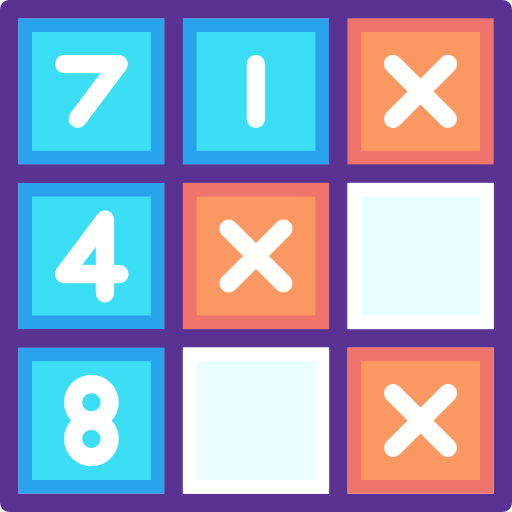
\includegraphics[scale=0.05]{sudoku.png} \bf Sudoku Game}
\date{2017.9}
\author{计64~~翁家翌~~2016011446}
\begin{document}
\kaishu
\ttfamily
\maketitle
%\tableofcontents
%\newpage
\section{软件用途}
本软件是一个数独小游戏,使用Qt5编写,实现了数独游戏的快速生成、以及提供任意题目的解决方案。
\section{运行方式}
安装Qtcreater之后,将源代码拷贝至本机,源代码位于\url{https://git.thusaac.org/trinkle/sudoku-qt5}。运行Qtcreater直接编译即可。

Ubuntu下需要额外安装软件包qtmultimedia5-dev,进入目录之后运行 \uline{qmake -makefile;make;} 即可得到可执行文件 sudoku。
\section{功能介绍}
\subsection{使用帮助}
\begin{figure}[htp]
\centering
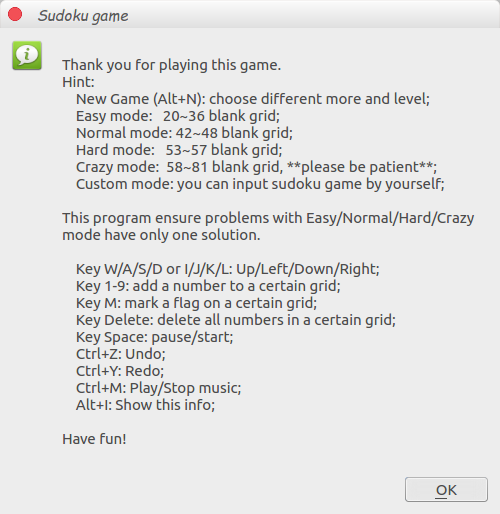
\includegraphics[width=0.5\linewidth]{help.png}
\caption{提示信息}
\label{fig:help}
\end{figure}

图~\ref{fig:help} 显示了关于本软件的使用帮助。它是运行软件时的最初界面,点击\uline{OK}即可进入主游戏界面。
\subsection{游戏界面}

\begin{figure}[htp]
\centering
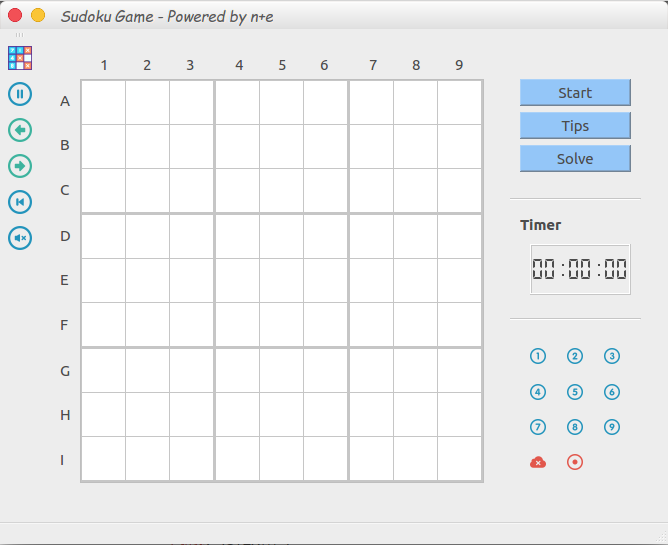
\includegraphics[width=0.7\linewidth]{start.png}
\caption{开始界面}
\label{fig:start}
\end{figure}

图~\ref{fig:start} 显示了软件的开始游戏界面。最上方为选项栏,左侧是菜单栏,中部是数独界面,右上侧是功能栏,右中部是计时器,右下侧是数字栏。

\subsection{选项栏}
\begin{figure}[htp]
\centering
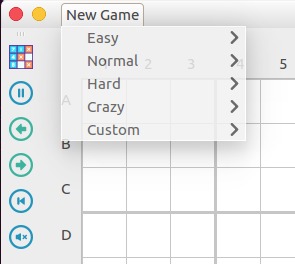
\includegraphics[width=0.5\linewidth]{title.png}
\caption{标题选项栏}
\label{fig:title}
\end{figure}

图~\ref{fig:title} 显示了软件的标题选项栏,{\bf 有四种难度可供选择,每种难度下有内置4个关卡,并且还有按照该难度随机生成题目的选项。

最后一个选项Custom提供了输入题目的功能,该软件能够给出用户提供题目的解答。}
\subsection{菜单栏}
\begin{figure}[htp]
\centering

\includegraphics[width=0.05\linewidth]{menubar.png}
\caption{菜单栏}
\label{fig:menu}
\end{figure}

图~\ref{fig:menu} 显示了软件的左侧菜单栏,从上到下依次为:显示信息(快捷键:\uline{Alt+I})、{\bf 暂停/继续游戏}(快捷键:\uline{空格})、{\bf 撤销}(快捷键:\uline{Ctrl+Z})、{\bf 重做}(快捷键:\uline{Ctrl+Y})、回到初始题目状态、{\bf 音效开关}(快捷键:\uline{Ctrl+M})。
\subsection{功能栏}
\begin{figure}[htp]
\centering
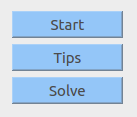
\includegraphics[width=0.3\linewidth]{function.png}
\caption{功能栏}
\label{fig:func}
\end{figure}

图~\ref{fig:func} 显示了软件的右上侧功能栏,从上到下依次为:开始游戏、{\bf 显示帮助}、{\bf 显示计算机给出的解答}。

显示帮助时,软件会显示一个还未被正确填上数字的格子的答案;显示帮助和解答时,均不会覆盖用户记录,下一步操作会回到点击按钮之前的状态。
\subsection{数字栏}
\begin{figure}[htp]
\centering

\includegraphics[width=0.2\linewidth]{number.png}
\caption{数字栏}
\label{fig:num}
\end{figure}

图~\ref{fig:num} 显示了软件的数字栏,点击$1\sim 9$(或者按下数字$1\sim 9$按键)即可在当前选中的格子上标记/去除一个点击的数字。第四行第一个图标为{\bf 清除一个格子内的所有数字}(快捷键:\uline{Delete}),第二个图标为{\bf 标记/取消标记一个选中的格子}(快捷键:\uline{M})。
\subsection{数独界面}
\begin{figure}[htp]
\centering
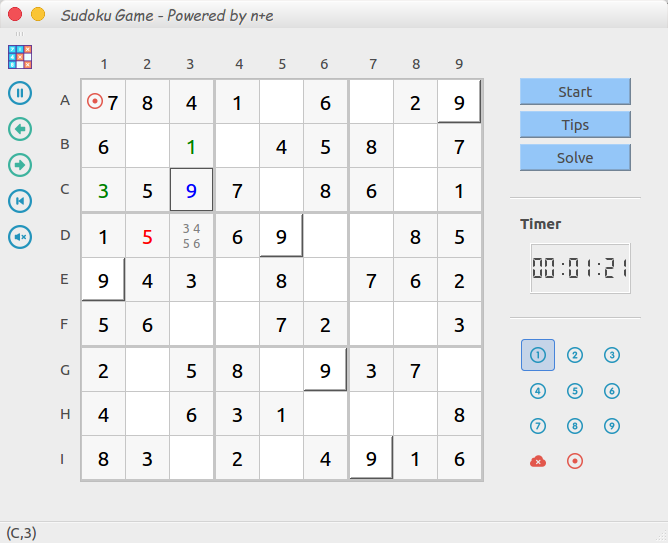
\includegraphics[width=1\linewidth]{status.png}
\caption{运行界面}
\label{fig:status}
\end{figure}

图~\ref{fig:status} 显示了软件在游戏过程中的运行界面。在每个时刻,均有一个格子被选中,用黑框蓝色字体高亮显示。当选中的格子已经填上一个数字,那么所有相同数字的格子均会{\bf 立体高亮}显示;否则如果选中的是一个空白格子,那么与这个格子同行同列的所有格子都会被{\bf 立体高亮}显示。当前选中格子的坐标在左下角会给予显示。

如果一个格子是题目数据,那么它会被标记为黑色字体;如果一个格子里有多个数字,那么程序将会以灰色小字号在格子内显示这些数字;如果一个填写上去的数字和已有数字{\bf 发生冲突},则{\bf 标记为红色字体};否则标记为绿色字体。

\begin{figure}[htp]
\centering
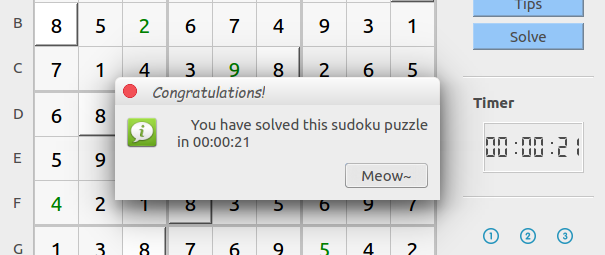
\includegraphics[width=0.7\linewidth]{finish.png}
\caption{完成解题}
\label{fig:finish}
\end{figure}

图~\ref{fig:finish} 显示了软件在用户完成解题时的界面。

\begin{figure}[htp]
\centering
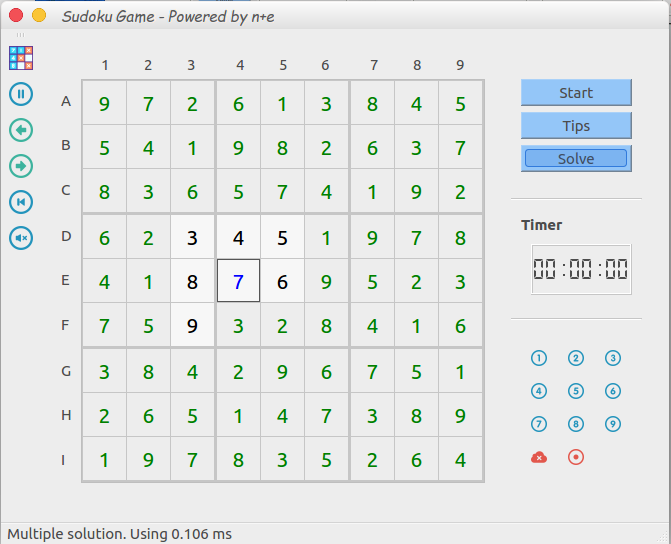
\includegraphics[width=0.7\linewidth]{solve.png}
\caption{自动解题}
\label{fig:solve}
\end{figure}

图~\ref{fig:solve} 显示了软件在Custom模式中按下 \fbox{Solve} 按钮之后的自动解题情况,黑色为用户输入数据,{\bf 左下角状态栏会显示是否多解/单解/无解,以及计算机解题的用时。}

\begin{figure}[htp]
\centering

\includegraphics[width=0.5\linewidth]{ewm.png}
\caption{有关数独算法的一个PDF}
\label{fig:ewm}
\end{figure}

\section{数独算法实现}

高中的时候仔细研究了一下数独的解法,发现Dancing Link完全可以被普通的搜索所取代。基本的思路是预处理出来一个搜索序列,然后用二进制表示的状态直接进行搜索。预处理出来的序列整体上保证是限制数目从小到大的,这样的话搜索树就会长得非常瘦,也更容易寻找到解。在\uline{[NOIP2009]靶型数独}一题中,这个方法比Dancing Link快一倍以上。并且本机测试,10000组数独题目,每组平均56.5空格,总计算时间为0.82秒。

有关这个算法的详细阐述,详见图~\ref{fig:ewm}。

\section{Qt界面实现}

界面设计的一个原则是,看起来要很清楚,感觉舒服,不要太多颜色花花绿绿的,感觉很浮夸,就像那种垃圾应用一样,玩着玩着给你开个广告。我尽量避免了给使用者留下这样的印象。

我使用了\uline{QTableWidget}创造出一个表单,再将81个\uline{QPushButton}嵌到表单里面。在设计的时候,我将所有的QpushButton的setFlat设置为True。这样的话扁平效果就能够体现。一个附带的效果就是,setFlat在True和False之间切换时,由于表单上的网格线,会使整个界面产生3D立体效果(误打误撞(x)。

有一个问题困扰了我很久:QPushButton在设置成扁平化之后,在选中的时候会出现蓝色的选中框,并且会影响上下左右键的原始操作。解决方案是将{\bf 所有的}QPushButton的setFocusPolicy改成\uline{Qt::NoFocus}即可。

在每次用户产生鼠标/键盘事件时,由于无需考虑界面的实现效率,因此为了方便,每个事件产生之后都会重新刷新一遍整个界面;并且一个好处就是,可以在刷新的时候顺便更新历史版本记录。

界面设计的另一个原则就是用户友好,每种操作既可以用鼠标也可以用键盘,在撤销/恢复/显示提示/显示解答/回到最初的时候都不会丢失之前的数据,所有历史数据都存储在一个\uline{QVector}中,每次要撤销/重做的时候直接移动指针,不会将原来已经在QVector中的数据删除,新一步的操作会append到QVector中,此时再使用撤销操作会回到上一次撤销前的状态。

在Qt程序中,我保存了四个$9\times 9$的数组,分别为:题目,解答,用户数字数据和用户标记数据。

代码很丑啊我只把数独算法和ui隔离开了,一点也不OO是吧但是写得爽233。
\end{document}